% Software Development for Mobile Devices
\documentclass[11pt,english,numbers=endperiod,parskip=half]{scrartcl}

\usepackage{color}
\usepackage{graphicx}
\usepackage{minted}
\usepackage{fancyhdr}
\usepackage{pdflscape}

\pagestyle{fancy}

\rhead{Daniel Parker - 971328X}
\lhead{COS30017 - Software Development for Mobile Devices}

\title{Assignment 08}
\subtitle{COS30017 - Software Development for Mobile Devices}
\author{Daniel Parker 971328X}

\date{\today}

\begin{document}
\maketitle
\thispagestyle{empty}

\section{Task 1}
\subsection{Introduction}
\subsection{Performance Optimisations}
\subsection{Usability Improvement}
\subsection{References}
\subsection{Appendix}

\section{Task 2}
This improved suntime app contains various new features including custom locations
using a map, sun rise and set times for a range of dates, and share functionality
to send a specific day's sun rise and set times for a location.

The new app includes the following fragments:
\begin{itemize}
	\item{List of preset locations}
	\item{Custom location using map}
\end{itemize}

\subsection{Screenshots}
\setlength\fboxsep{0pt}
\setlength\fboxrule{0.5pt}

\begin{figure}[H]
\centering{
	\fbox{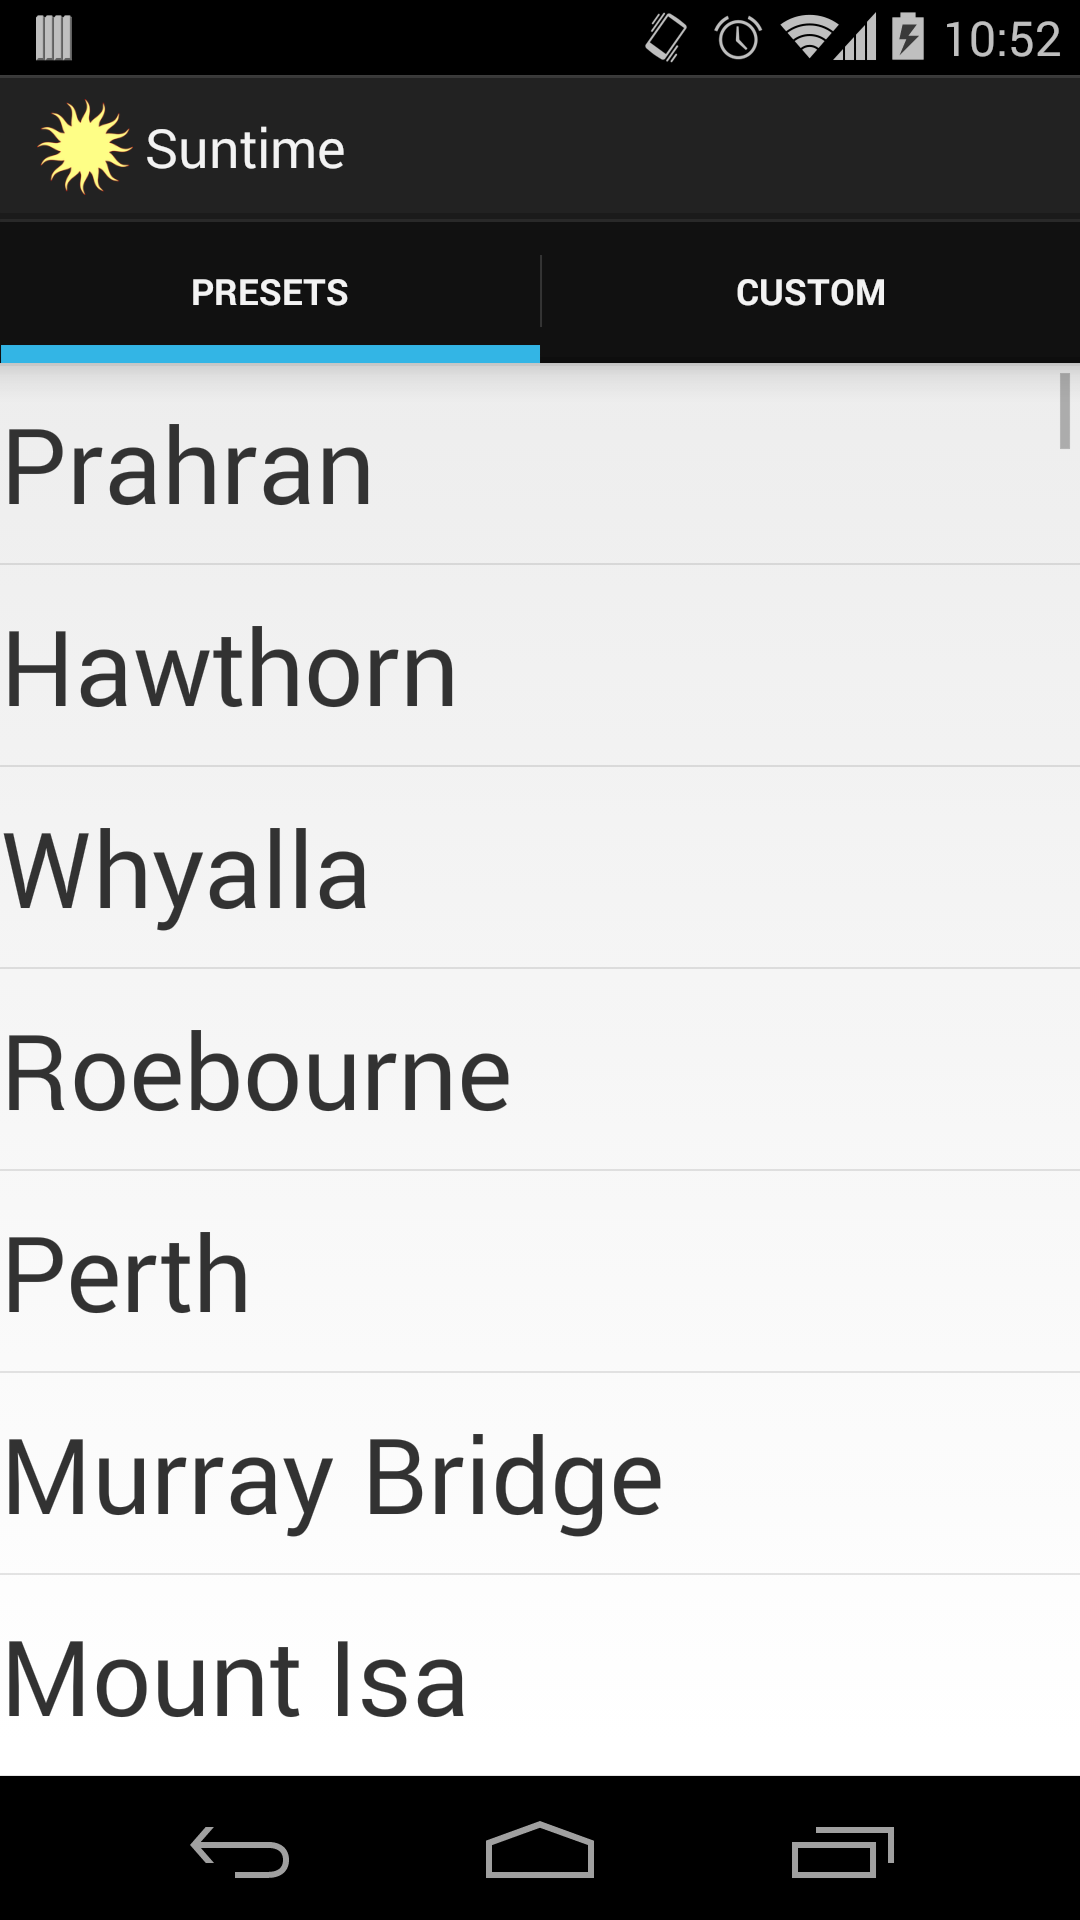
\includegraphics[width=5cm]{images/preset.png}}
}\\
\end{figure}

\begin{figure}[H]
\centering{
	\fbox{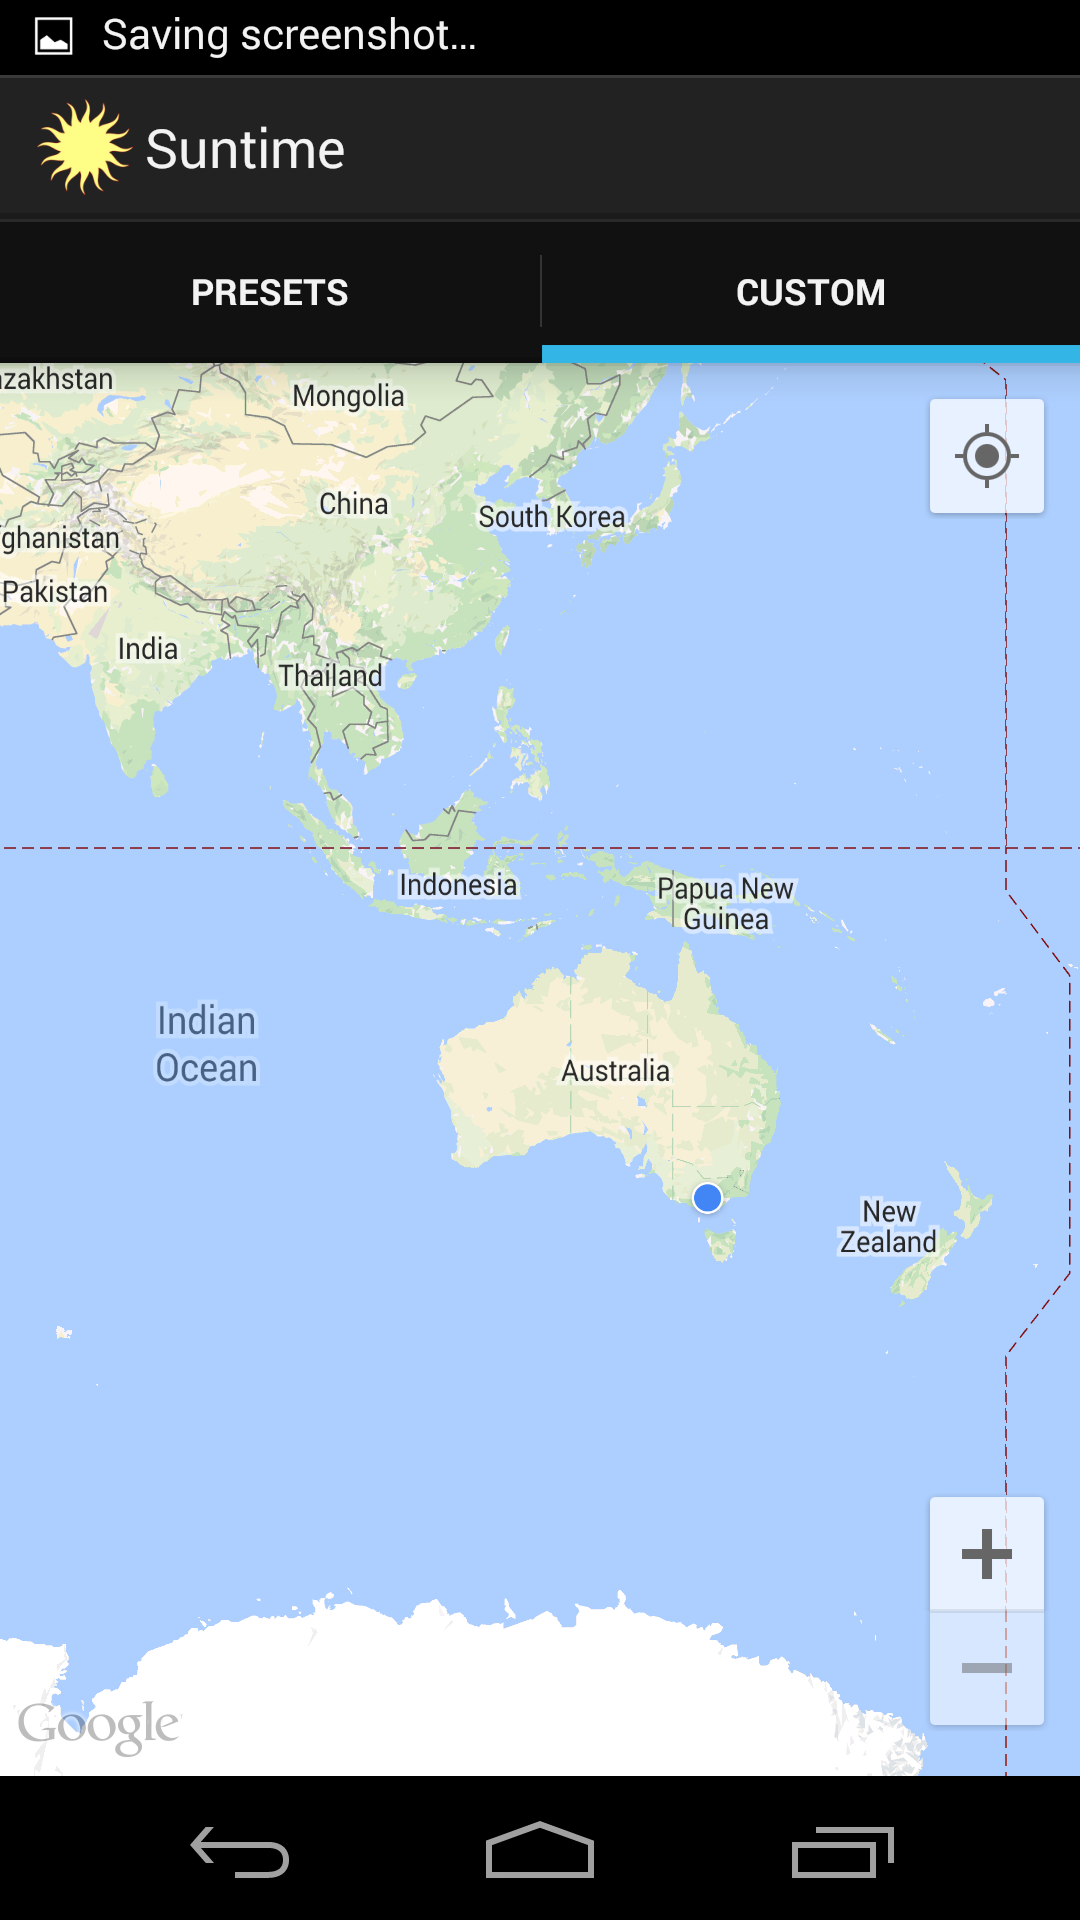
\includegraphics[width=5cm]{images/map.png}}
}\\
\end{figure}

\begin{figure}[H]
\centering{
	\fbox{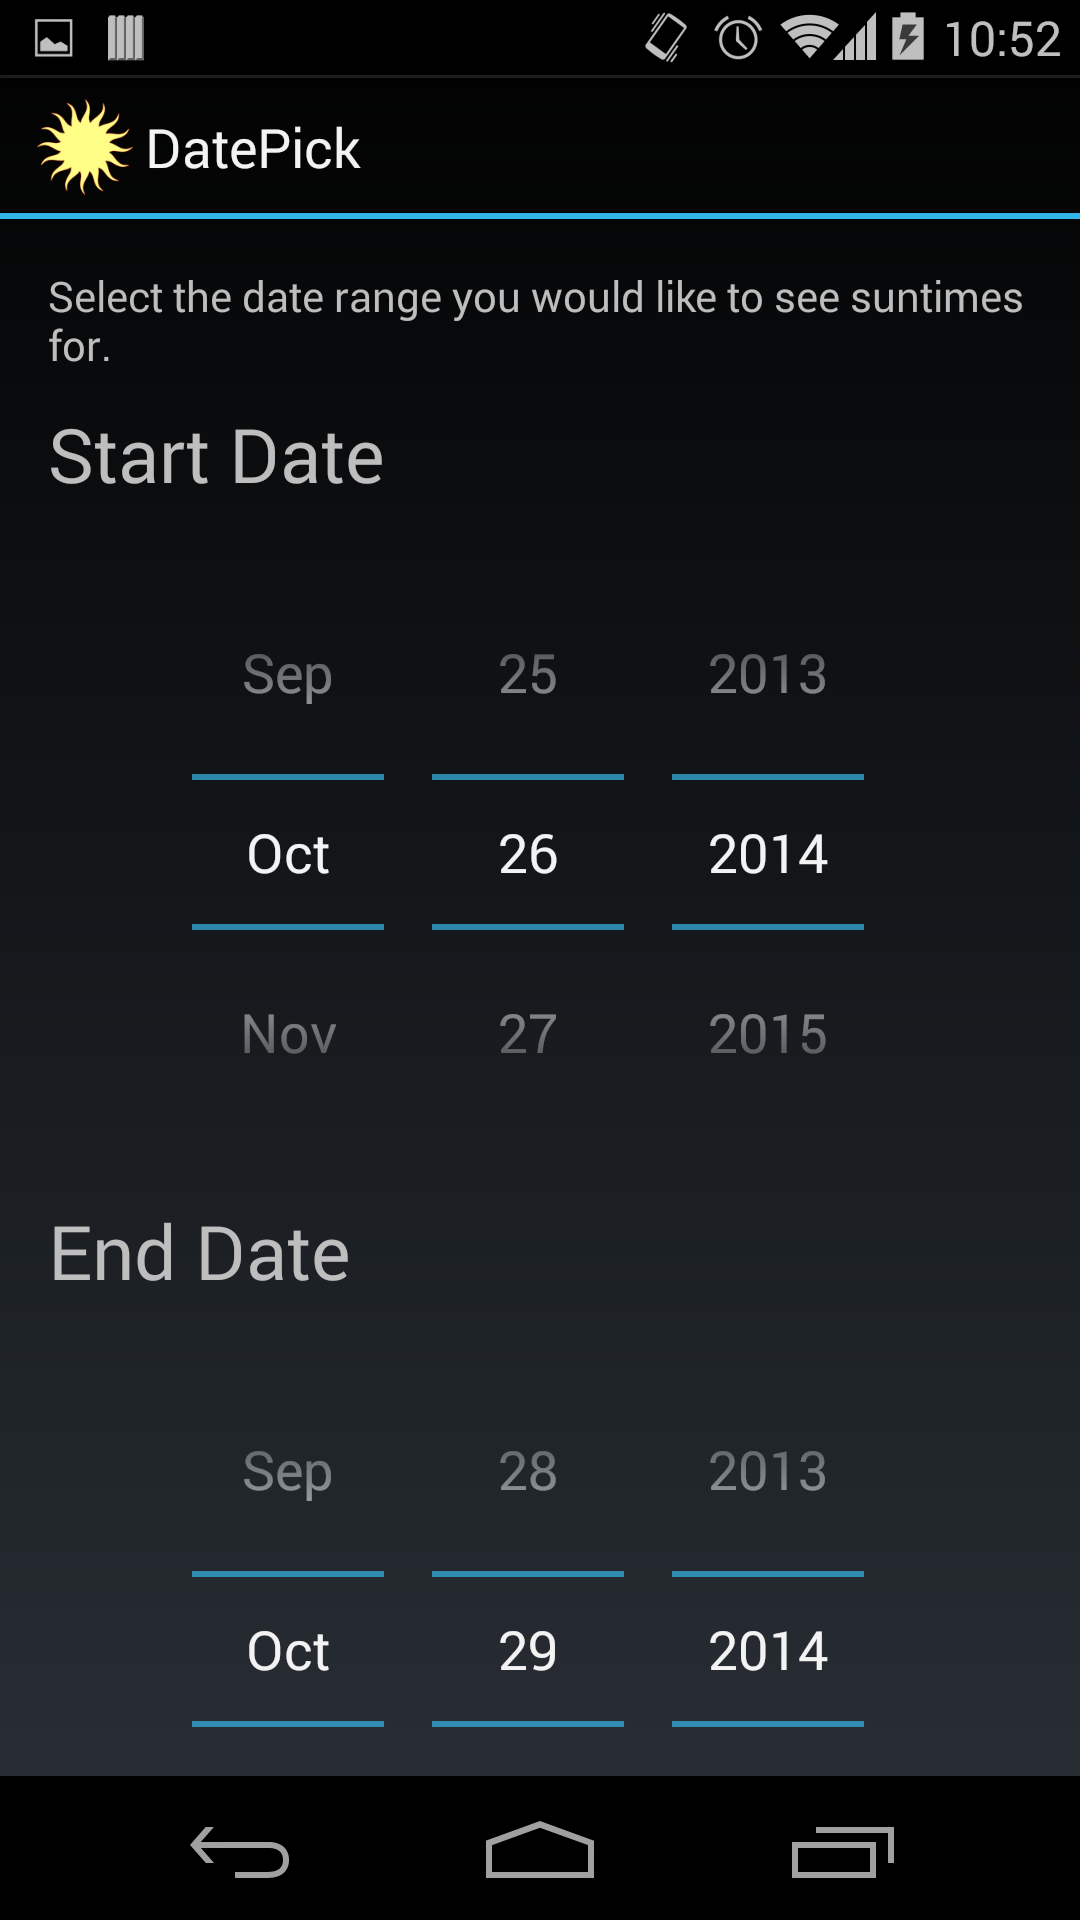
\includegraphics[width=5cm]{images/range.png}}
}\\
\end{figure}

\begin{figure}[H]
\centering{
	\fbox{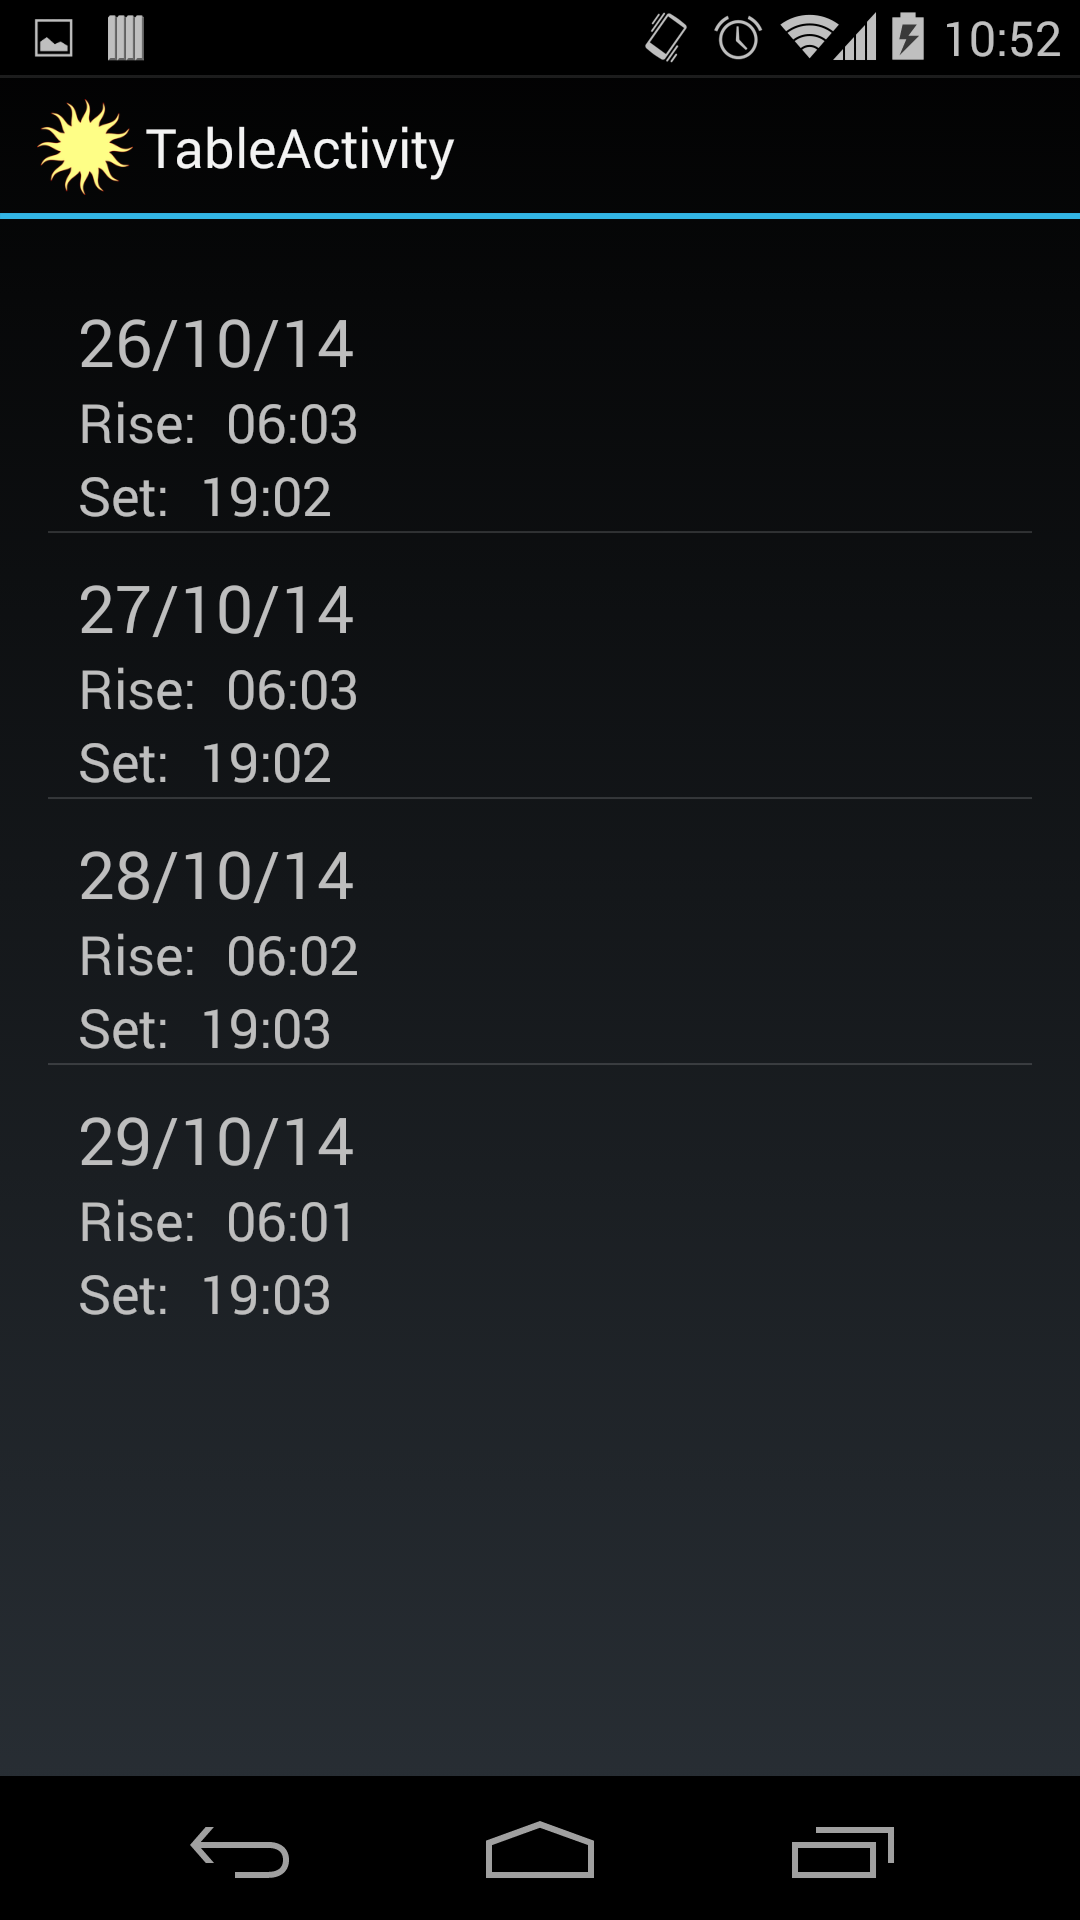
\includegraphics[width=5cm]{images/table.png}}
}\\
\end{figure}

\begin{figure}[H]
\centering{
	\fbox{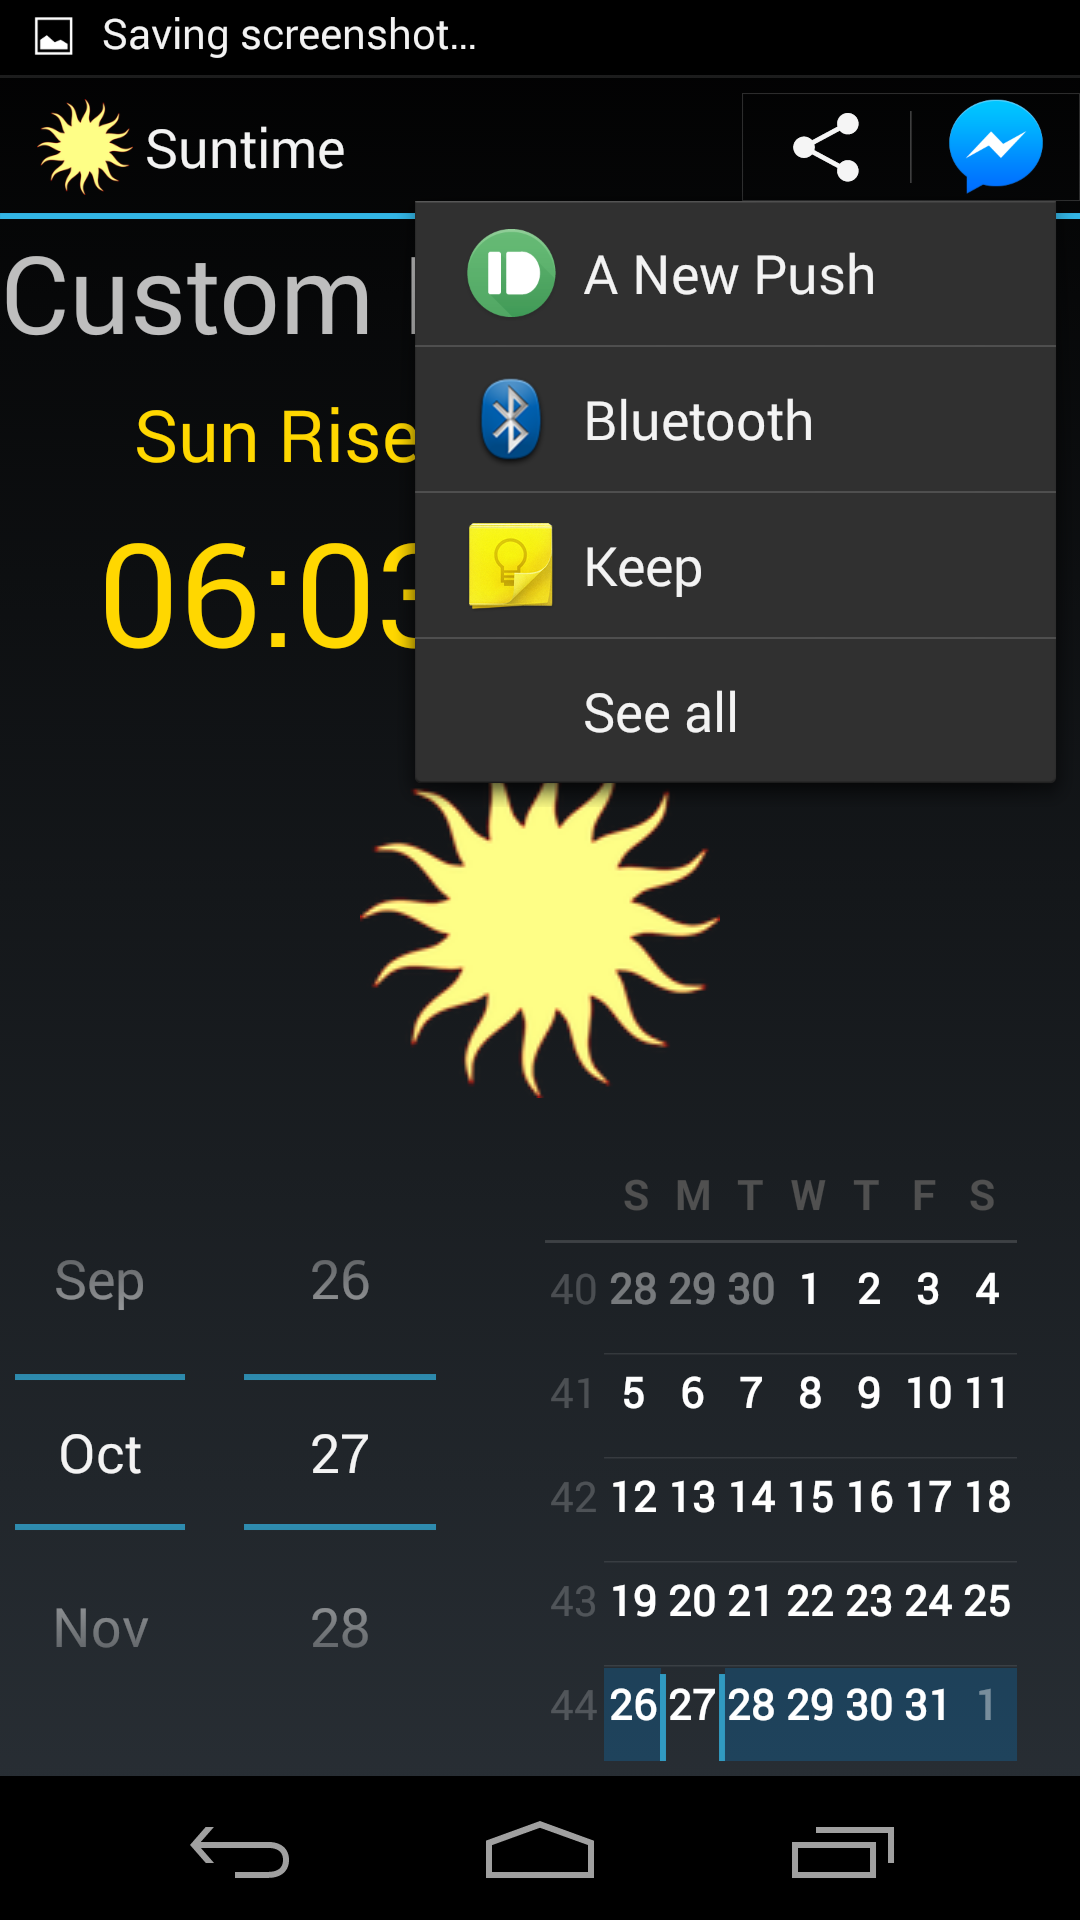
\includegraphics[width=5cm]{images/share.png}}
}\\
\end{figure}
\begin{landscape}
\subsection{Source}
\subsubsection{MainActivity}
\inputminted[firstline=17, lastline=82]{java}{../../Apps/FinalSuntime/app/src/main/java/au/net/danielparker/suntime/ui/MainActivity.java}

\subsubsection{CustomFragment}
\inputminted[firstline=28, lastline=89]{java}{../../Apps/FinalSuntime/app/src/main/java/au/net/danielparker/suntime/ui/CustomFragment.java}


\end{landscape}
\end{document}
